\documentclass[border=10pt]{standalone}

\usepackage{tikz}
\usepackage{tikzsymbols}
\usetikzlibrary{calc,patterns,shapes.geometric}

\def\centerarc[#1](#2)(#3:#4:#5){\draw[#1] ($(#2)+({#5*cos(#3)},{#5*sin(#3)})$) arc (#3:#4:#5);}

\begin{document}
	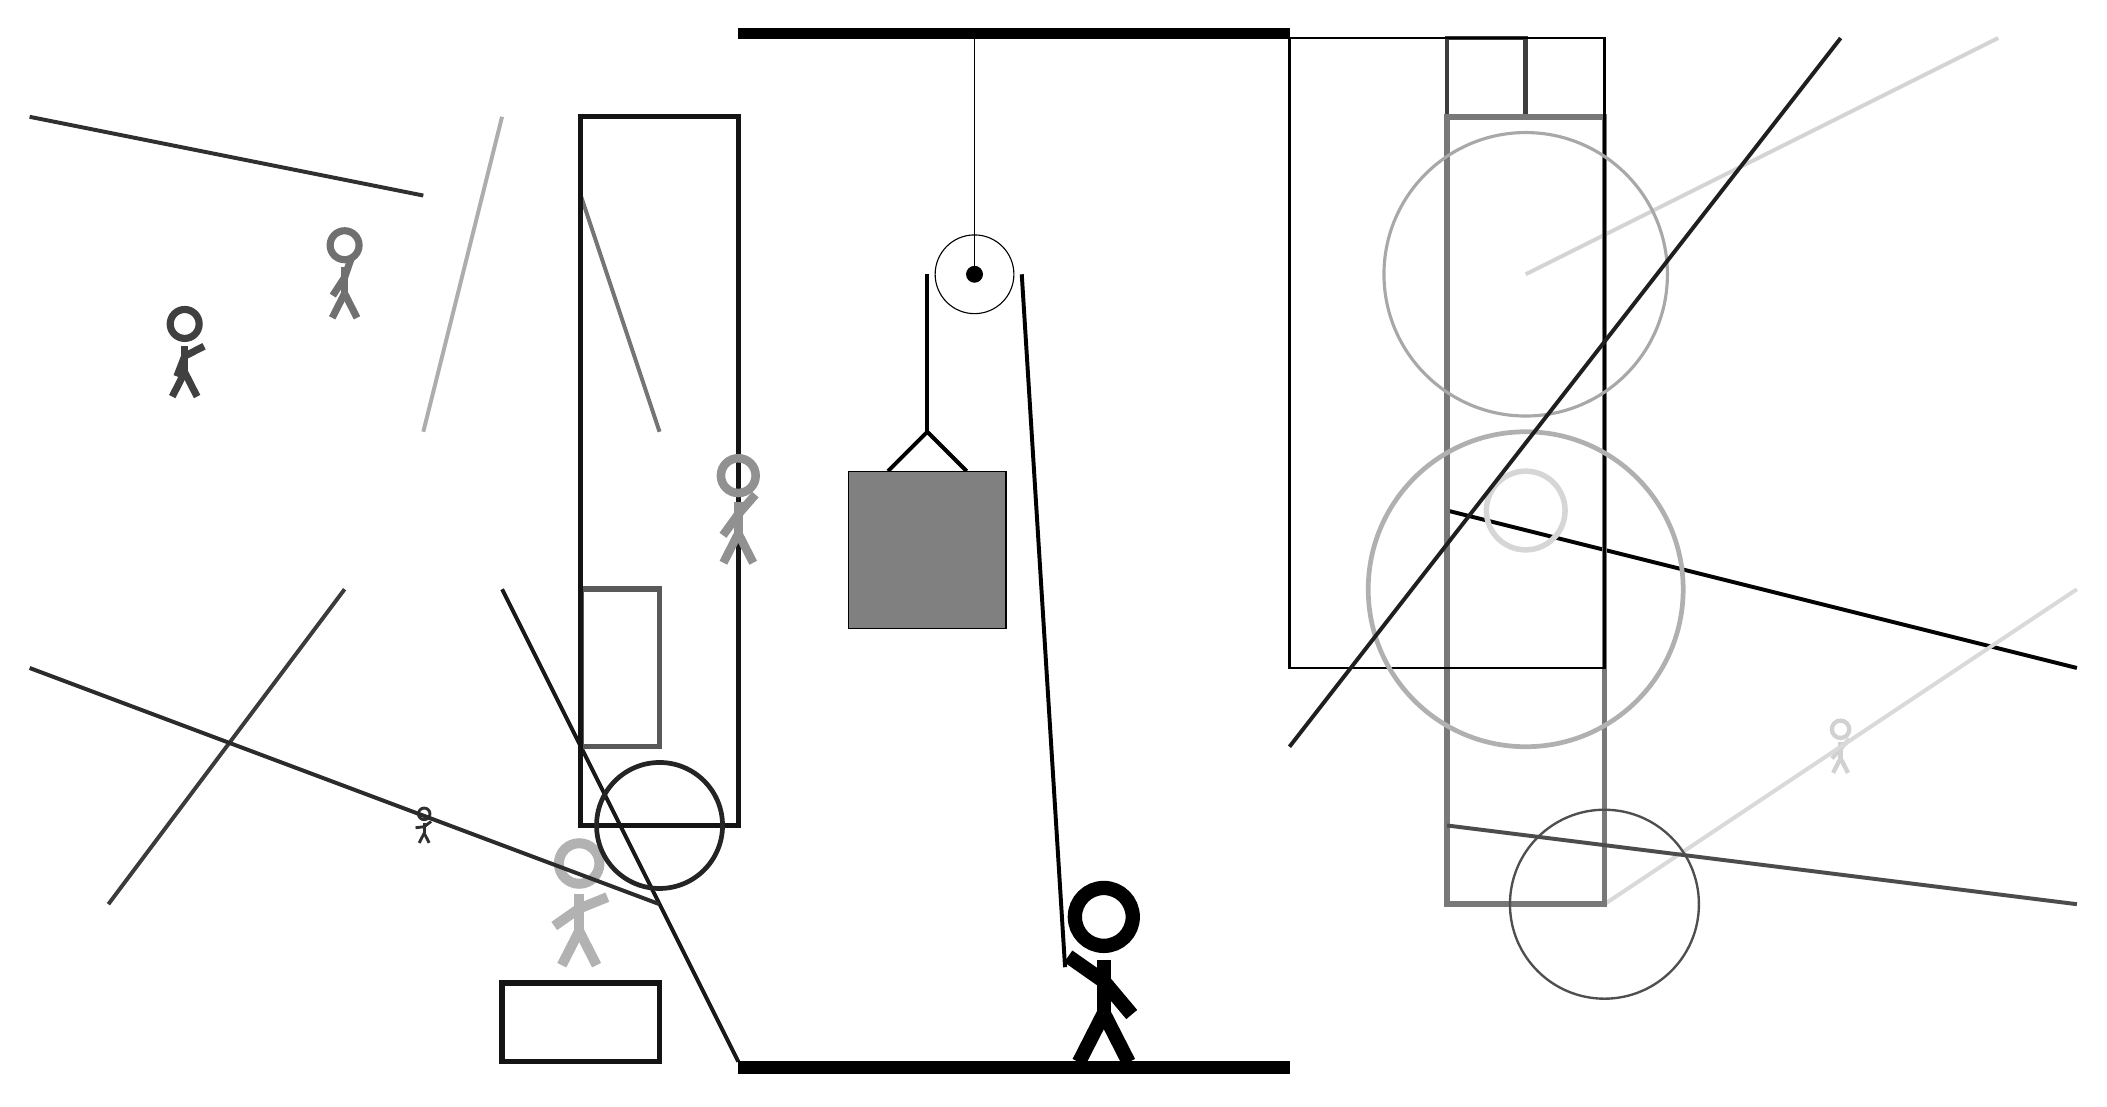
\begin{tikzpicture}
		%%%%% START %%%%%
		
		\draw[fill=black] (-2, 10) rectangle (5, 10.125);
		
		\draw (1, 7) circle (0.5);
		\draw[fill=black] (1, 7) circle (0.1);
		\draw (1, 10) -- (1, 7);
		
		\draw[line width=0.5mm] (-0.1, 4.5) -- (0.4, 5.0) -- (0.9, 4.5);
		\draw[fill=black!50] (-0.6, 4.5) rectangle (1.4, 2.5);
		
		\draw[line width=0.5mm] (0.4, 7) -- (0.4, 5.0);
		\centerarc[line width=0.5mm](1, 7)(0:180:0.6);
		\draw[line width=0.5mm](1.6, 7) -- (2.15, -1.8);
		
		\draw[line width=0.5mm, color=black!17](8, 7) -- (14, 10);
		
		\node[line width=0.7mm, color=black!81] at (-6, 0) {\Strichmaxerl[2][7][37]};
		\draw[line width=0.5mm, color=black!90](-2, -3) -- (-5, 3);
		\draw[line width=0.5mm, color=black!77](-7, 3) -- (-10, -1);
		\node[line width=0.6mm, color=black!30] at (-4, -1) {\Strichmaxerl[7][35][22]};
		
		\draw[line width=0.5mm, color=black!83](-3, -1) -- (-11, 2);
		
		\node[line width=0.6mm, color=black!18] at (12, 1) {\Strichmaxerl[3][49][47]};
		
		\draw[line width=0.5mm, color=black!99](7, 4) -- (15, 2);
		\draw[line width=0.7mm, color=black!65] (-3, 1) rectangle (-4, 3);
		\draw[line width=0.5mm, color=black!54](-4, 8) -- (-3, 5);
		\draw [line width=0.7mm, color=black!16](8, 4) circle (0.5);
		\draw[line width=0.5mm, color=black!15](9, -1) -- (15, 3);
		\draw[line width=0.6mm, color=black!76] (7, 9) rectangle (8, 10);
		
		\draw[line width=0.7mm, color=black!53] (7, -1) rectangle (9, 9);
		\draw[line width=0.6mm, color=black!92] (-4, 0) rectangle (-2, 9);
		\draw[line width=0.3mm, color=black!100] (5, 10) rectangle (9, 2);
		
		\draw [line width=0.4mm, color=black!34](8, 7) circle (1.8);
		\draw [line width=0.3mm, color=black!69](9, -1) circle (1.2);
		\draw[line width=0.5mm, color=black!70](7, 0) -- (15, -1);
		\draw [line width=0.6mm, color=black!31](8, 3) circle (2.0);
		\draw[line width=0.5mm, color=black!81](-6, 8) -- (-11, 9);
		
		\draw[line width=0.7mm, color=black!92] (-3, -3) rectangle (-5, -2);
		\node[line width=0.5mm, color=black!56] at (-7, 7) {\Strichmaxerl[5][57][71]};
		\draw[line width=0.5mm, color=black!88](5, 1) -- (12, 10);
		\draw [line width=0.6mm, color=black!86](-3, 0) circle (0.8);
		\draw[line width=0.5mm, color=black!32](-5, 9) -- (-6, 5);
		\node[line width=0.4mm, color=black!75] at (-9, 6) {\Strichmaxerl[5][69][27]};
		\node[line width=0.7mm, color=black!43] at (-2, 4) {\Strichmaxerl[6][54][49]};
		
		\node at (2.6, -1.9) {\Strichmaxerl[10][-35][-50]};
		
		\draw[fill=black] (-2, -3) rectangle (5, -3.15);
		
		%%%%% END %%%%%
	\end{tikzpicture}
\end{document}